\documentclass[../../ASSD_TP1_G7.tex]{subfiles}
\begin{document}
\chapter*{Muestreo sub-Nyquist}
El muestreo sub-Nyquist se utiliza para se\~nales acotadas en banda con el espectro fuera de la Banda base. Para analizar este tipo de muestreo se utilizo una se\~nal AM, ya que su espectro coincide con las característica deseada.
\begin{equation}
X_c=A_{Max}[\frac{1}{2}cos(2\pi (1.8 f_{in})t)+cos(2\pi (2 f_{in})t)+cos(2\pi (2.2 f_{in})t)]
\end{equation}\label{eq:inputSignlan}

Donde $f_{in}= 36KHz$, entonces la frecuencia de la portadora es $72KHz$ y la modulada $7.2KHz$.
\section*{Rango de frecuencia de sampleo}
Definiendo $B$ al ancho de banda de la se\~nal y $f_c$ a la frecuencia central del espectro. El rango de frecuencias de sampleo $(f_s)$ es:
\begin{equation}
f_{sMIN}=\frac{2f_c + B}{m+1} < \frac{2f_c - B}{m} = f_{sMAX}
\end{equation}
Donde $m$ son las repeticiones del espectro. Conociendo $f_{in}$ y la se\~nal AM, $B=14.4KHz$ y $f_c=72KHz$.

\begin{table}[htbp]
\begin{center}
\begin{tabular}{|l|l|l|}
\hline
$m$ & $f_{sMIN}$ & $f_{sMAX}$  \\
\hline \hline
2 & $52.8KHz$ & $64.8KHz$ \\ \hline
3 & $39.6KHz$ & $43.2KHz$ \\ \hline
4 & $31.7KHz$ & $32.4KHz$ \\ \hline
\end{tabular}
\caption{Frecuencias de Sampleo}
\label{tabla:fsamp}
\end{center}
\end{table}
Para $m$ mayores, $f_{sMIN}>f_{sMAX}$.

\section*{Mediciones}
Las mediciones se realizaron para el caso de $m=2$.

Utilizando la frecuencia de sampleo m\'inima (figuras \ref{fig:subnyq_lla_fmin} y \ref{fig:subnyq_syh_fmin}), se observa que las dos r\'eplicas del espectro original (en verde y rojo) est\'an lado a lado. El pico de frecuencia m\'axima de la repetici\'on verde se encuentra superpuesto con el pico de frecuencia m\'inima de la repetici\'on roja, por lo que no se pueden diferenciar en el diagrama espectral. En consecuencia, entre ambas repeticiones deber\'ian medirse 5 picos. 

Con la frecuencia de sampleo media (figuras \ref{fig:subnyq_lla_fmed} y \ref{fig:subnyq_syh_fmed}), tanto el espectro original (en celeste) como las dos repeticiones (en verde y rojo) se encuentran separados, por lo que no hay picos superpuestos. En consecuencia, 9 picos deber\'ian ser visibles. 

Si la frecuencia de sampleo es la m\'axima, (figuras \ref{fig:subnyq_syh_fmax} y \ref{fig:subnyq_lla_fmax}), el pico superior de la repetici\'on roja coincide con el pico inferior de el espectro original.



\subsection*{Llave Analógica}
\begin{figure}[H]
\centering
\subcaptionbox{Simulación}
{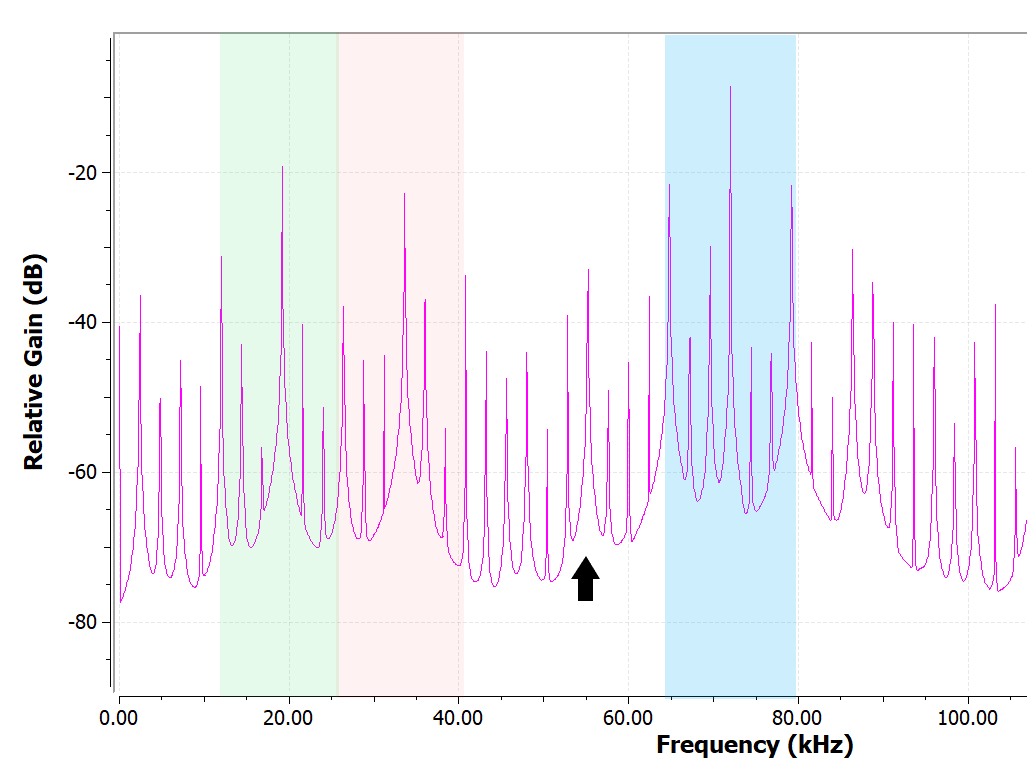
\includegraphics[width=0.6\textwidth]{figures/simpto_8_llave_52,8khz_espectro.png}}
\subcaptionbox{Medición}
{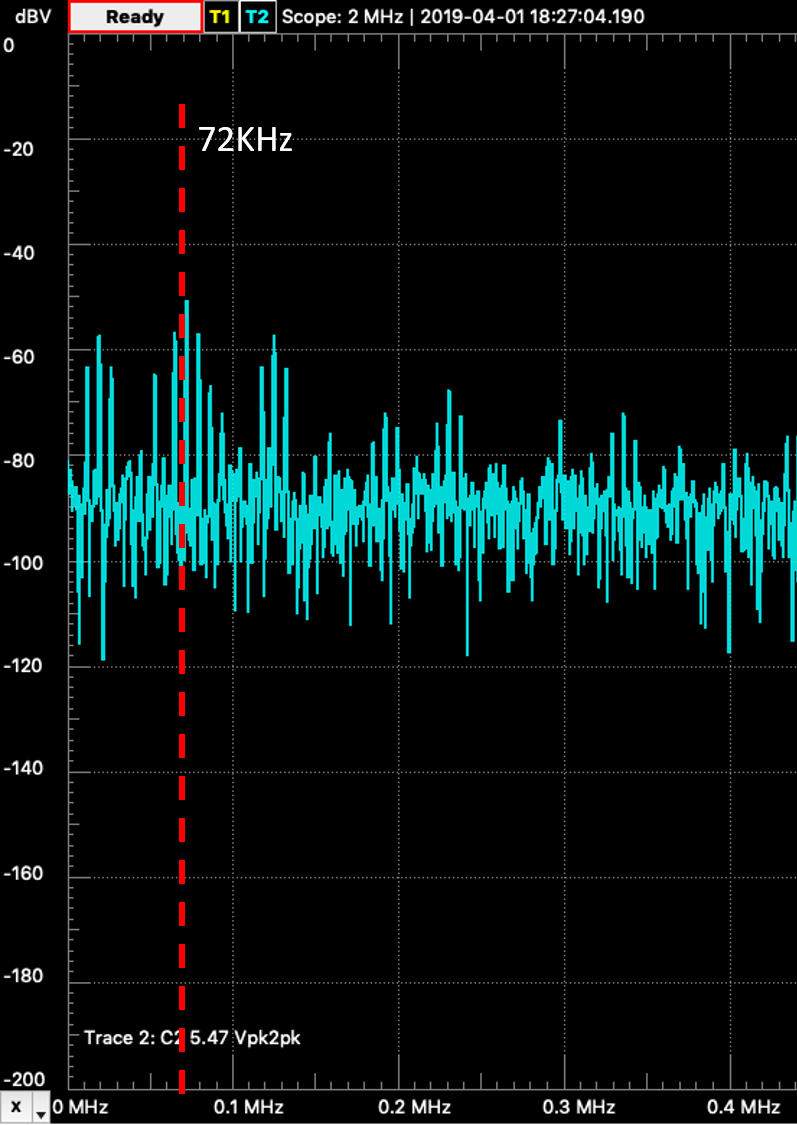
\includegraphics[width=0.32\textwidth]{figures/pto_8_llave_52,8khz_espectro.png}}
\caption{Frecuencia sampleo mínima(52.8KHz), simulación y medición}
\label{fig:subnyq_lla_fmin}
\end{figure}

\begin{figure}[H]
\centering
\subcaptionbox{Simulacion}
{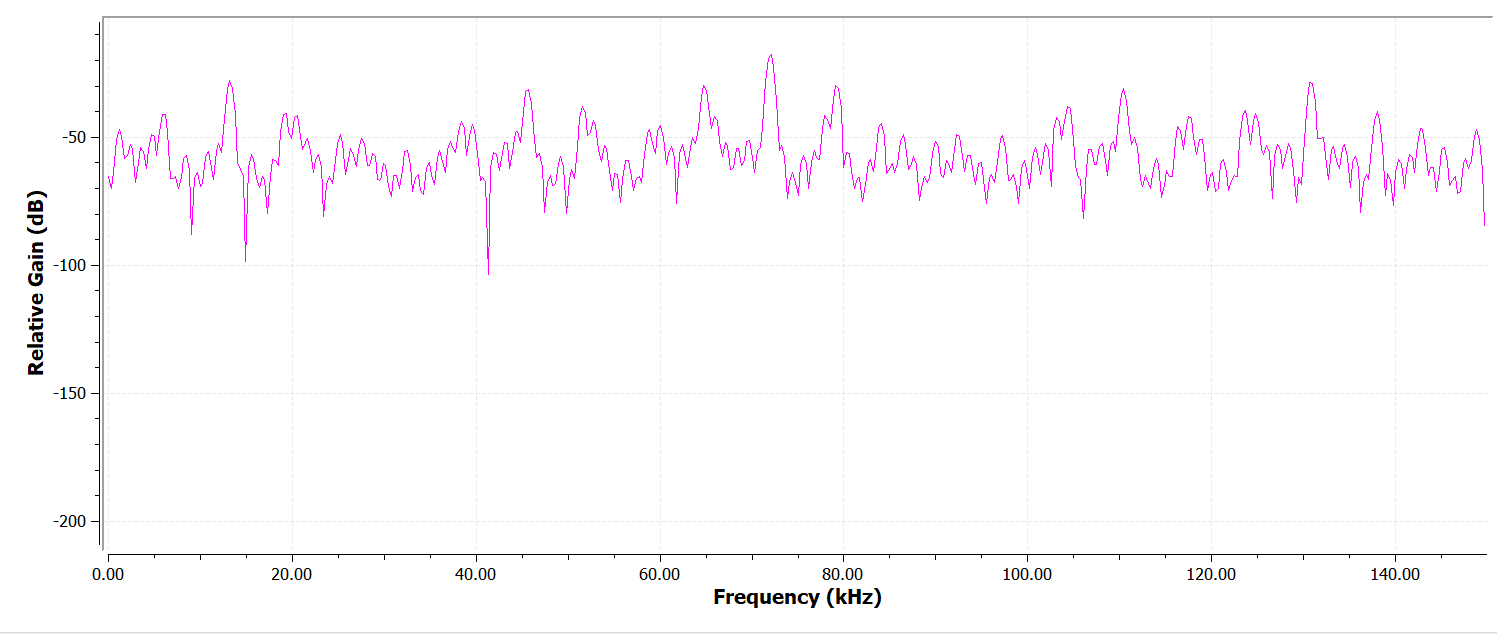
\includegraphics[width=0.6\textwidth]{figures/simpto_8_llave_58,8_espectro.png}}
\subcaptionbox{Medicion}
{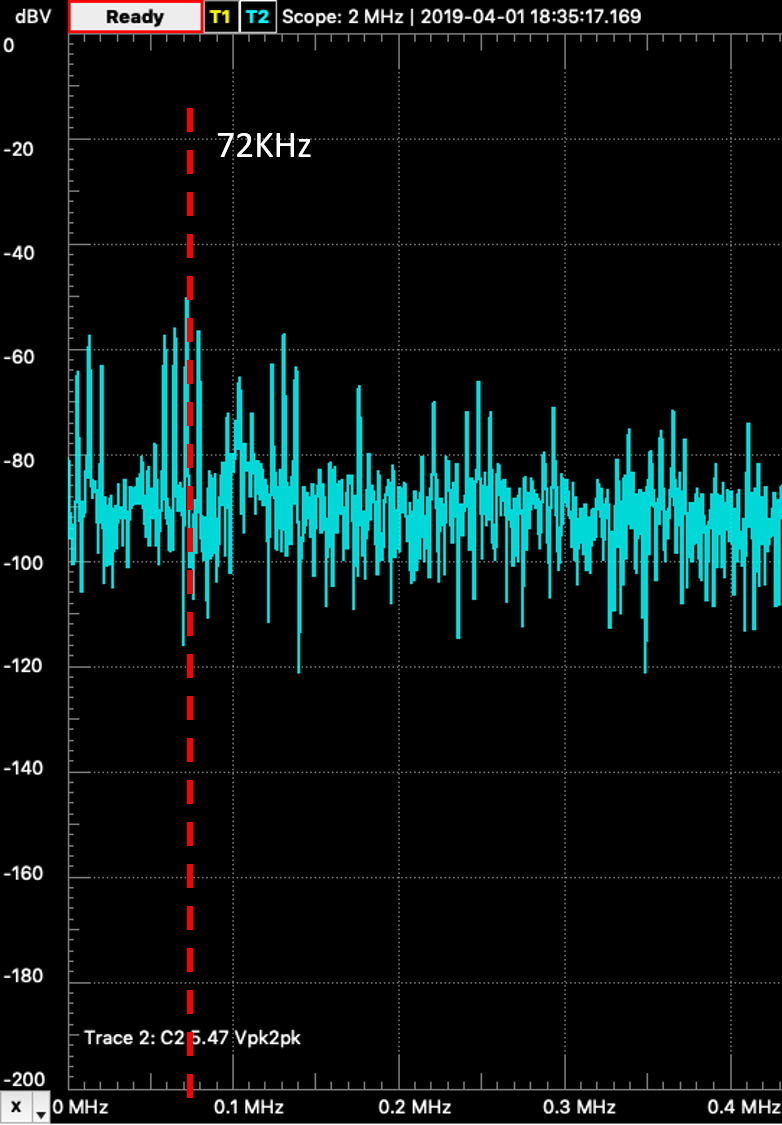
\includegraphics[width=0.32\textwidth]{figures/pto_8_llave_58,8_espectro.png}}
\caption{Frecuencia sampleo media(58.8KHz), simulación y medición}
\label{fig:subnyq_lla_fmed}
\end{figure}

\begin{figure}[H]
\centering
\subcaptionbox{Simulación}
{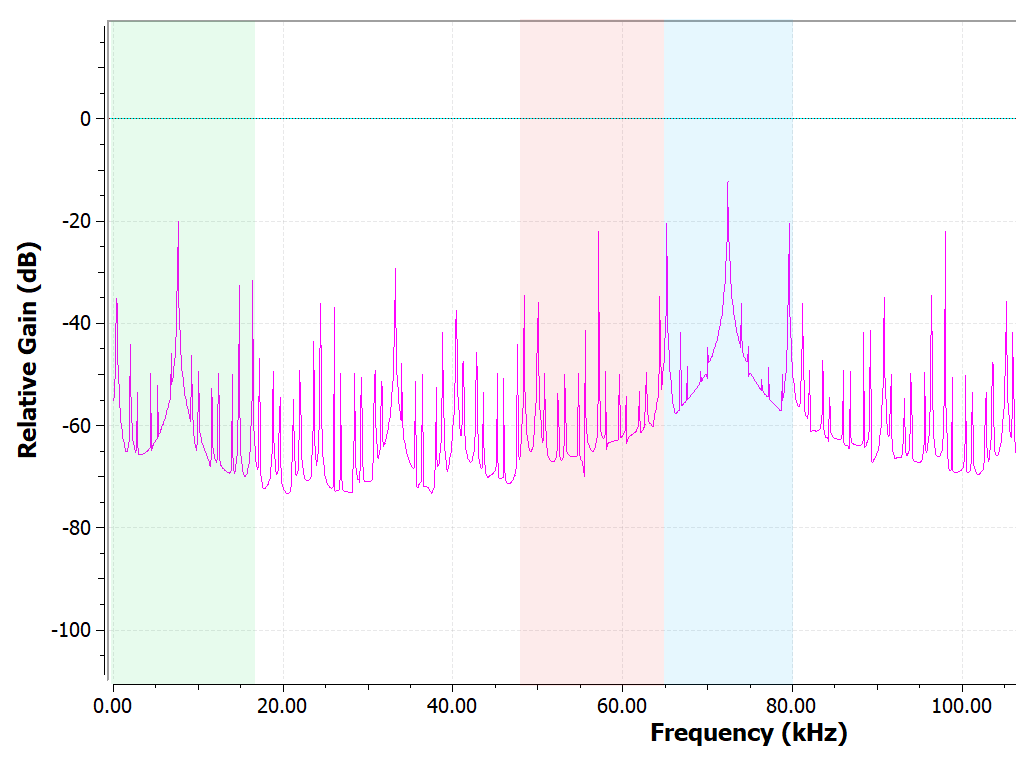
\includegraphics[width=0.6\textwidth]{figures/simpto_8_llave_64,8khz_espectro.png}}
\subcaptionbox{Medición}
{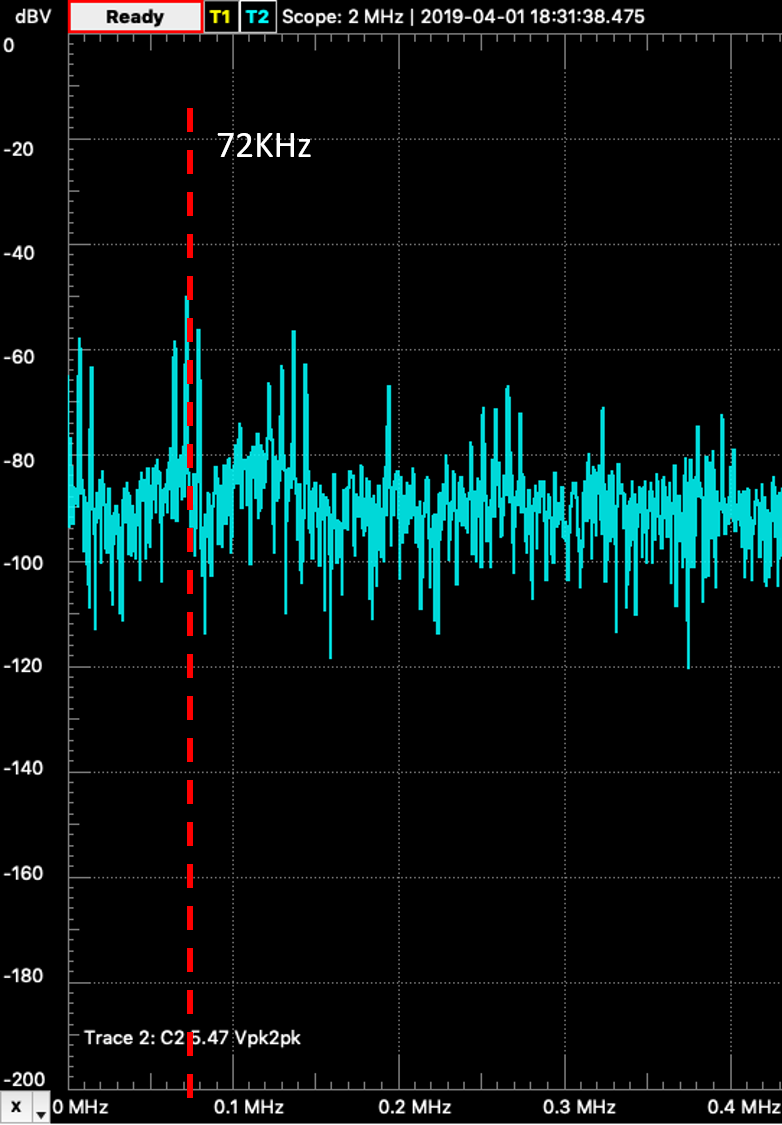
\includegraphics[width=0.32\textwidth]{figures/pto_8_llave_64,8khz_espectro.png}}
\caption{Frecuencia sampleo maxima(64.8KHz), simulación y medición}
\label{fig:subnyq_lla_fmax}
\end{figure}


\subsection*{Sample and Hold}
\begin{figure}[H]
\centering
\subcaptionbox{Simulación}
{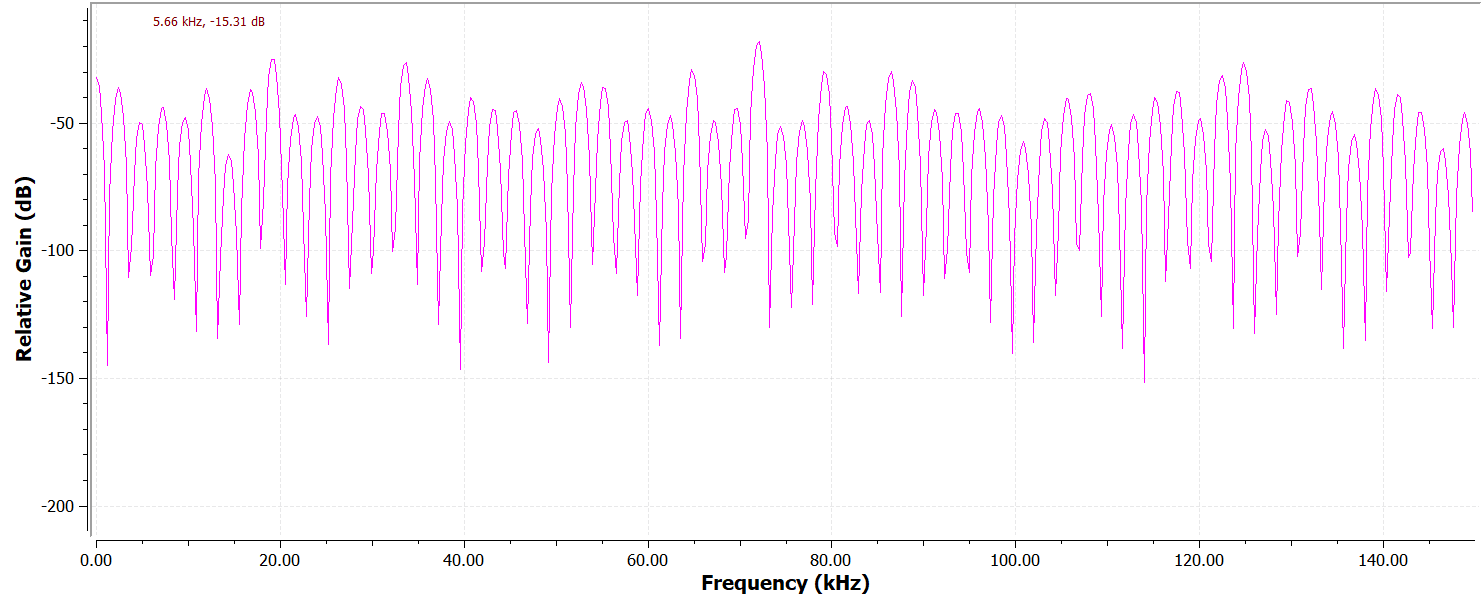
\includegraphics[width=0.6\textwidth]{figures/simpto_8_syh_52,8_espectro.png}}
\subcaptionbox{Medición}
{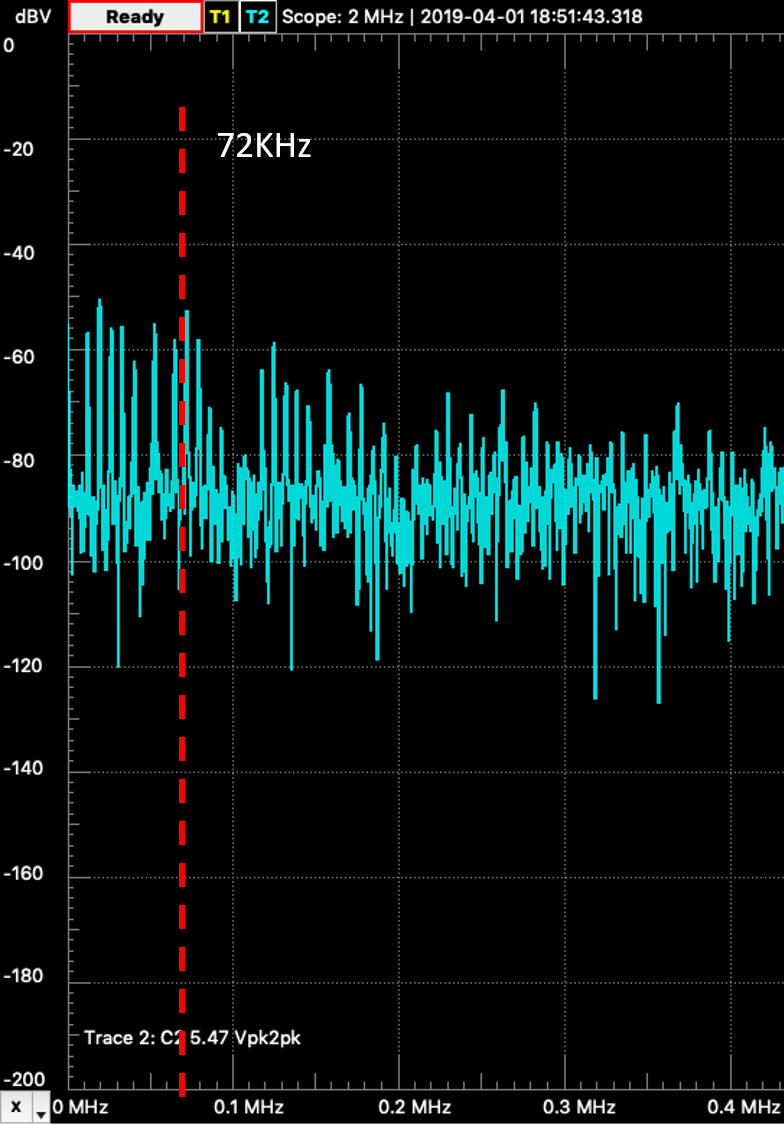
\includegraphics[width=0.32\textwidth]{figures/pto_8_syh_52,8_espectro.png}}
\caption{Frecuencia sampleo mínima(52.8KHz), simulación y medición}
\label{fig:subnyq_syh_fmin}
\end{figure}

\begin{figure}[H]
\centering
\subcaptionbox{Simulacion}
{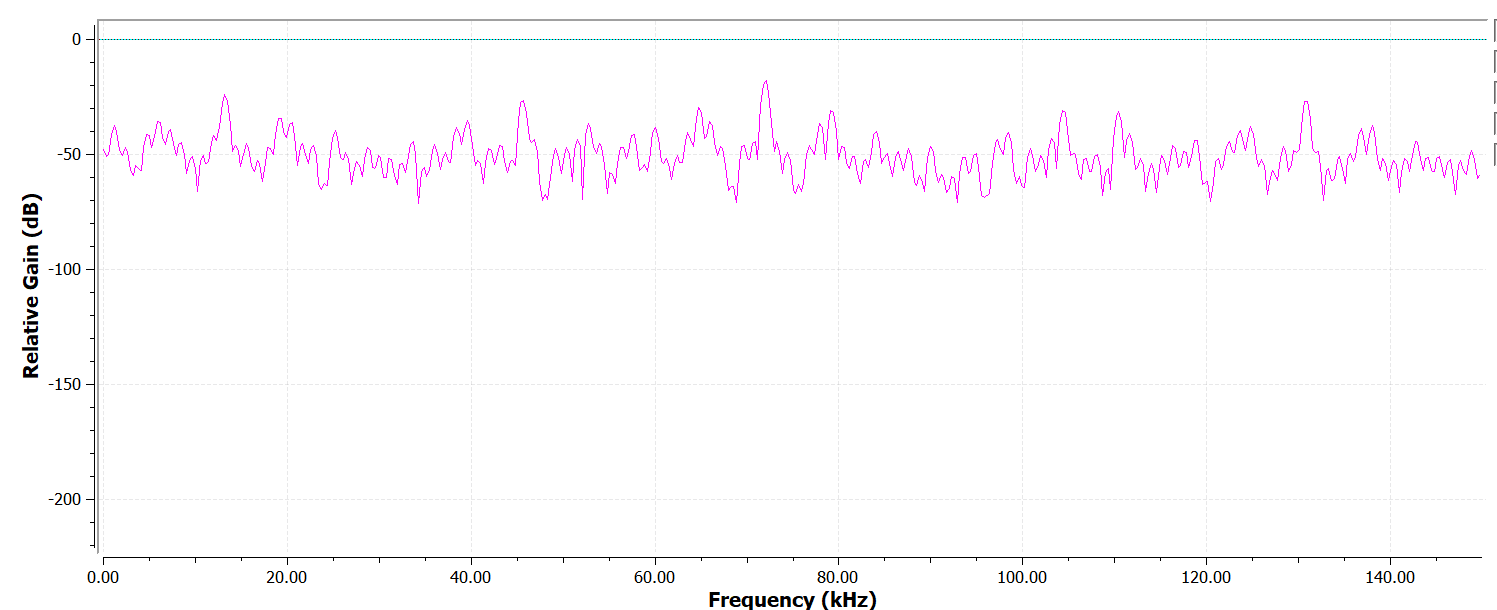
\includegraphics[width=0.6\textwidth]{figures/simpto_8_syh_58,8_espectro.png}}
\subcaptionbox{Medicion}
{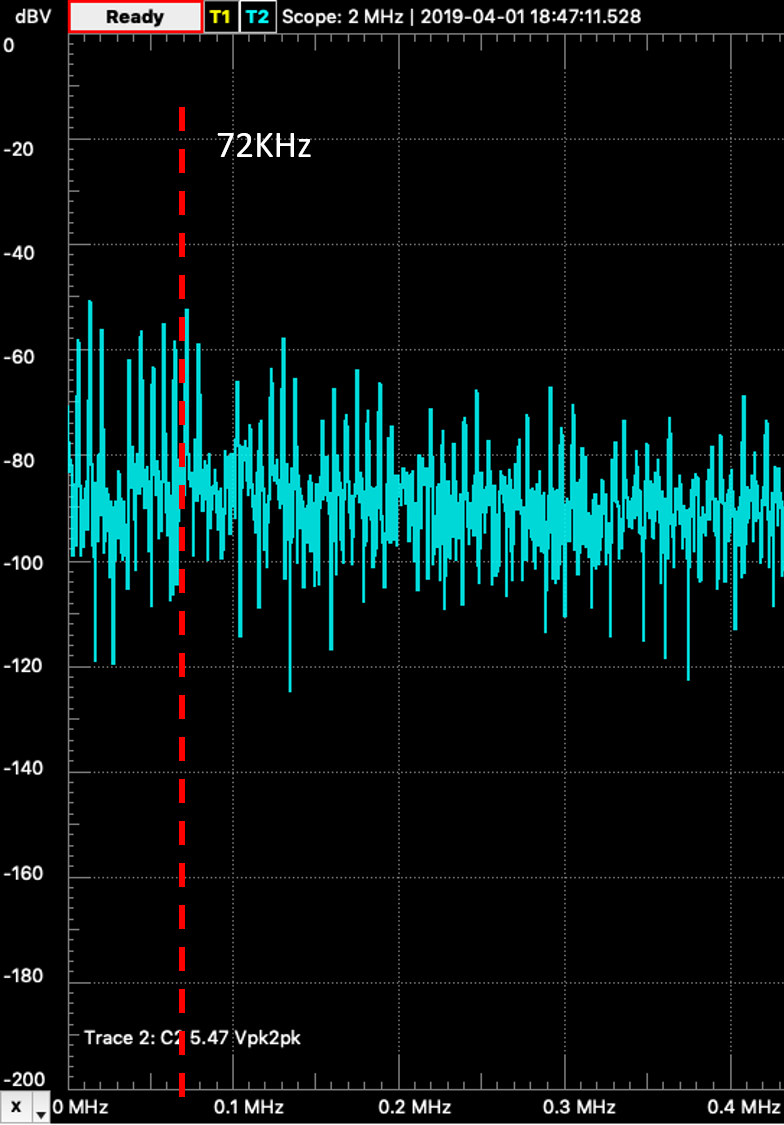
\includegraphics[width=0.32\textwidth]{figures/pto_8_syh_58,8_espectro.png}}
\caption{Frecuencia sampleo media(58.8KHz), simulación y medición}
\label{fig:subnyq_syh_fmed}
\end{figure}

\begin{figure}[H]
\centering
\subcaptionbox{Simulación}
{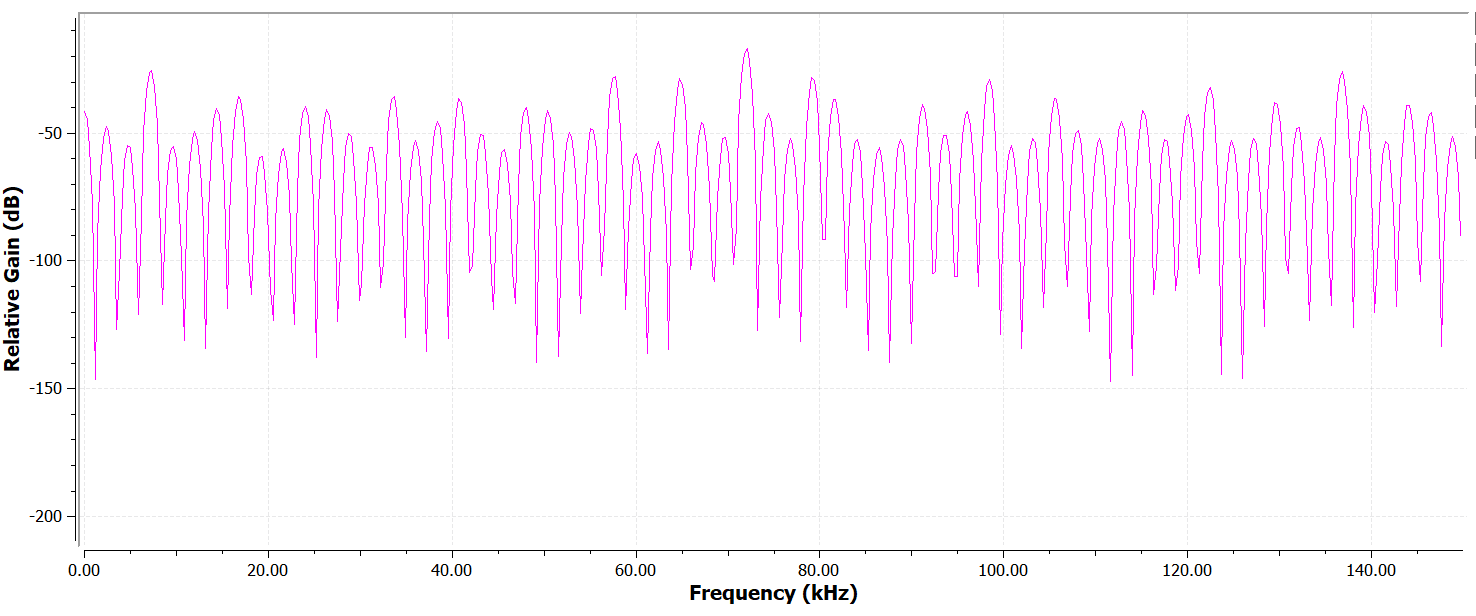
\includegraphics[width=0.6\textwidth]{figures/simpto_8_syh_64,8_espectro.png}}
\subcaptionbox{Medición}
{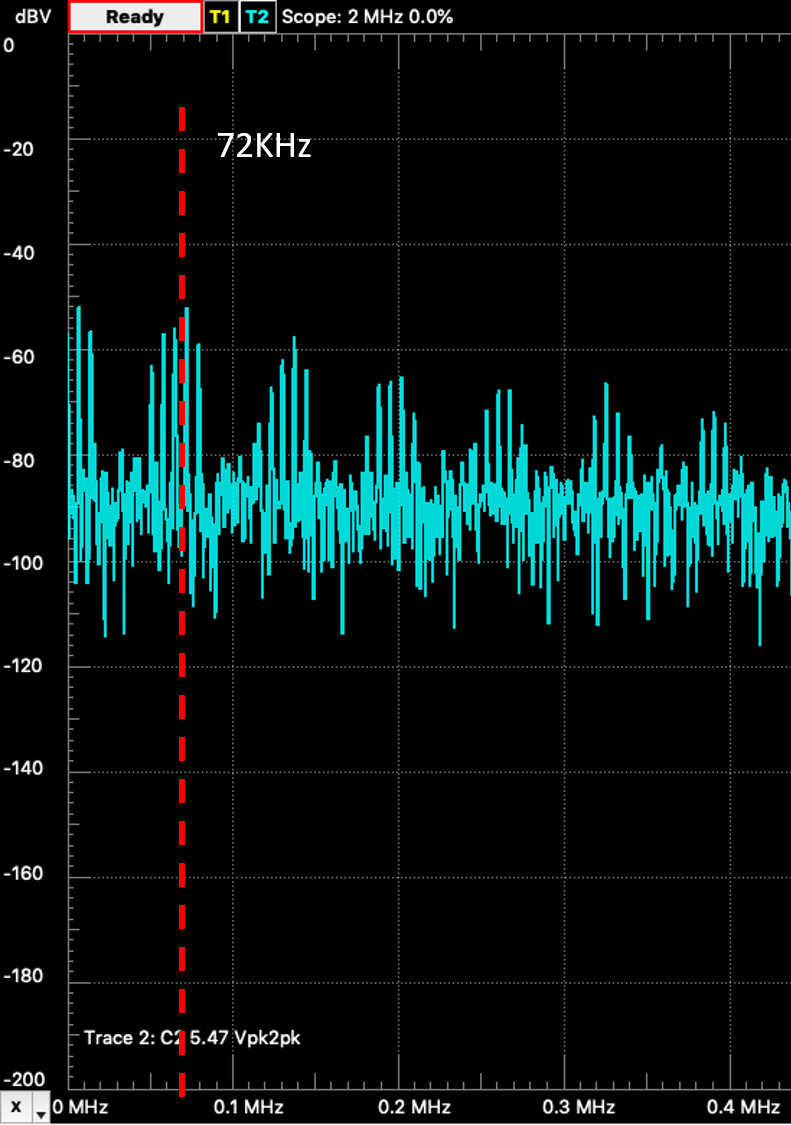
\includegraphics[width=0.32\textwidth]{figures/pto_8_syh_64,8_espectro.png}}
\caption{Frecuencia sampleo maxima(64.8KHz), simulación y medición}
\label{fig:subnyq_syh_fmax}
\end{figure}

\subsection*{Recuperación de la se\~nal}
Se intento recuperar la se\~nal proveniente de la llave analógica, para ello se conecto el filtro recuperador. Se obtuvo la siguiente medición:

\begin{figure}[H]
  \centering
   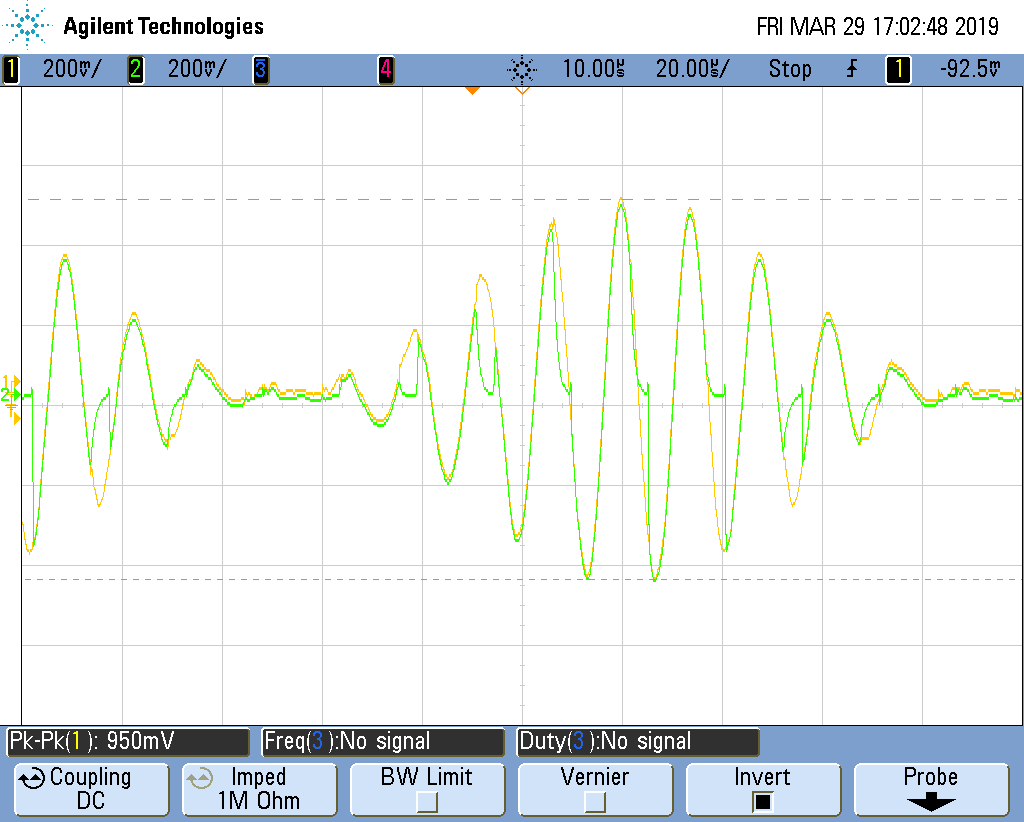
\includegraphics[width=0.7\textwidth]{figures/lla_8_1.png}
  \caption{Recuperación de la se\~nal. Canal amarillo entrada, canal verde salida }
  
\end{figure}
Tal como se observa en la imagen, no fue posible la recuperación, esto se deve a que el filtro recuperador es un pasabajos y no un pasa banda. Entonces no se filtran las repeticiones del espectro.


\end{document}
